\section{The Automatic Identification System (AIS) dataset}

AIS (Automatic Identification System) was developed in the 1990s to enhance navigation safety and prevent ship collisions.
It allows ships equipped with AIS to communicate with each other and coastal authorities through VHF transmissions.
The International Maritime Organization (IMO) mandates that all international voyage ships above 300 gross tonnage and all passenger ships must have an AIS transmitter.
Governments and authorities in different nations also enforce AIS applications to improve safety and security.

\begin{figure}[h]
    \centering
    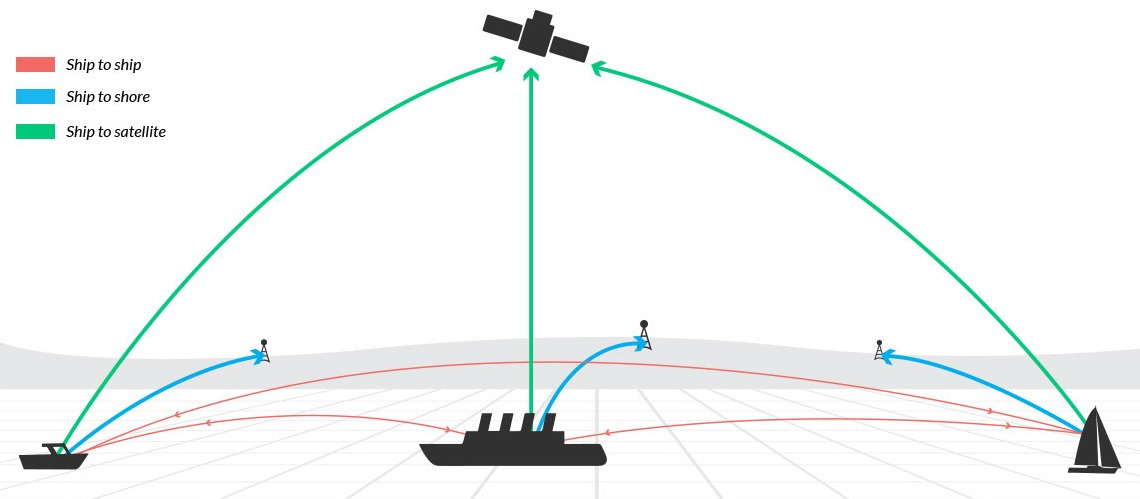
\includegraphics[width=0.7\textwidth]{images/ais.jpeg}
    \caption{Working of AIS}
    \label{ais}
\end{figure}

There are two types of AIS transceivers: Class A and Class B.
Class A transceivers broadcast more data fields and have higher reporting frequencies.
The information broadcasted by a Class A transceiver can be categorized into static information, dynamic information, and voyage-related information.
Dynamic information is automatically transmitted every 2-10 seconds when the ship is underway and every 3 minutes when anchored.
Static and voyage-related information are broadcasted every 6 minutes regardless of navigational status.
Class B transponders transmit a reduced set of data and have sparser reporting intervals compared to Class A transponders.


\begin{table}[ht]
    \centering
    \begin{tabular}{|l|l|p{0.5\linewidth}|}
        \hline
        \textbf{Data field}       & \textbf{Type} & \textbf{Description}                                                                      \\
        \hline
        AIS identity and location & Static        & Maritime Mobile Service Identity (MMSI) and the location of the system's antenna on board \\
        \hline
        Ship identity             & Static        & Ship name, IMO number, type, and call sign of the ship                                    \\
        \hline
        Ship size                 & Static        & Length and width of the ship                                                              \\
        \hline
        Ship position             & Dynamic       & Latitude and longitude (up to 0.0001 min accuracy)                                        \\
        \hline
        Speed                     & Dynamic       & Ranging from 0 knot to 102 knots (0.1 knot resolution)                                    \\
        \hline
        Rate of turn              & Dynamic       & Right or left (ranging from 0 to 720° per minute)                                         \\
        \hline
        Timestamp                 & Dynamic       & Timestamp of the message in UTC                                                           \\
        \hline
    \end{tabular}
    \caption{AIS message data fields \autocite{perez2009automatic}}
    \label{tab:ais_message}
\end{table}


Table \ref{tab:ais_message} shows the data fields transmitted by AIS messages.
Combining AIS data with other databases can provide additional information.
For example, port-to-port average speed can be calculated based on voyage distance and time stamps reported at the two ports.
Cargo weight can be estimated using draught and ship sizes. Technical ship specifications, such as DWT (deadweight tonnage), capacity, design speed, and design draught, can be obtained from fleet databases using the IMO number.
Port-to-port bunker consumption can be estimated based on speed, distance, and technical ship specifications like DWT and capacity \autocite{yang2019big}.


